\input{style/sqtbeamer.tex}

\title{Intro to Quant}
\subtitle{Workshop}
\institute{Sydney Quant Traders \\ $\times$ \\ UNSW Competitive Programming \& Mathematics Society}
\date{}

\begin{document}

\maketitle

\section{Trading \& Markets}

\begin{frame}{Motivation}
  We will introduce the concepts of
  \begin{itemize}
    \item trading
    \item exchanges
    \item the orderbook
  \end{itemize}

  \vspace{0.3cm}

  \textcolor{sqt-question}{
    I thought that firms don't care about prior knowledge of finance?
  }

  \begin{itemize}
    \item this is only true during the interview stage for large HFT firms
    \item beginner understanding of orderbook dynamics is useful for
    \begin{itemize}
      \item mock trading games
      \item general understanding of the industry
    \end{itemize}
  \end{itemize}
\end{frame}

\begin{frame}{Spot Trades}
  \begin{sqt:tip}
    Alice says to Bob:
    \begin{center}
      ``I want to to sell you 5 AAPL shares. Each share will be sold at \$30. 
      This transfer will occur by the end of the next business day (tomorrow)." 
    \end{center}
  \end{sqt:tip}

  This defines a \textbf{spot trade} (as opposed to a \textbf{future trade}).

  \begin{sqt:definition}
    A \textbf{spot trade} is an agreement to exchange assets for money, with 
    the actual transfer occuring almost immediately (within 1 or 2 business days).
    \begin{itemize}
      \item sides (Alice is selling, Bob is buying)
      \item quantity of the asset being traded ($5$)
      \item price per asset ($\$30$)
    \end{itemize}
  \end{sqt:definition}
\end{frame}

\begin{frame}{Trade Execution and Settlement}
  Once Bob \textbf{agrees} to this trade, the trade can be \textbf{executed}.

  \begin{sqt:definition}
    Upon trade \textbf{execution}, both parties are given \textbf{settlement obligations}.
  \end{sqt:definition}
  \begin{sqt:tip}
    For example, in Alice \& Bob's equity spot trade, the obligations are:
    \begin{itemize}
      \item Alice must give Bob $5$ shares of AAPL by the settlement deadline
      \item Bob must give Alice $5\times \$30 = \$150$ by the settlement deadline
    \end{itemize}
    Once the obligations are fulfilled, the trade is considered \textbf{settled}.
  \end{sqt:tip}

  Obligations on other asset classes and types of trades (e.g. futures and options) 
  are considerably more complex than this.
  Concepts related to \textbf{clearing} and \textbf{settlement} are 
  considered part of the \textbf{post-trade life-cycle}.
\end{frame}

% TODO: finish
\begin{frame}{Holdings and Position}
  At each point in time, each participant has a \textbf{holdings} and a \textbf{position} in each asset.

  \begin{center}
    TODO: insert diagram
  \end{center}

  \begin{sqt:definition}
    \textbf{Position} includes the effects of executed \textbf{trades} that have not been \textbf{settled} yet.
  \end{sqt:definition}

  \begin{sqt:result}
    Your exposure and PnL is determined by your \textbf{position}.
    % As a result, for trading games and simulations, we can abstract away the entire post-trade life-cycle
    % and just consider our \textbf{position}, disregarding \textbf{holdings} entirely.
  \end{sqt:result}
\end{frame}

\begin{frame}{What is an Exchange}
  \begin{sqt:definition}
    An \textbf{exchange} is a centralised venue for participants to\\
    find willing counterparties to make \textbf{trades} with.
  \end{sqt:definition}
  \begin{sqt:definition}
    If a trade does not occur on an exchange, then the trade is \textbf{over-the-counter} (OTC).
  \end{sqt:definition}
  \vspace{0.5cm}

  \begin{center}
    \begin{columns}
      \begin{column}[t]{0.3\textwidth}
        US exchanges
        \begin{itemize}
          \item (XNYS) NYSE
          \item (XNAS) Nasdaq
          \item (XCBO) CBOE
          \item (XCME) CME
        \end{itemize}
      \end{column}

      \begin{column}[t]{0.3\textwidth}
        APAC exchanges
        \begin{itemize}
          \item (XHKG) HKEX
          \item (XSHG) SSE
          \item (XSGE) SHFE
        \end{itemize}
      \end{column}
    \end{columns}
  \end{center}
\end{frame}

\begin{frame}{Counterparty Discovery}
  \begin{center}
    \textcolor{sqt-question}{
      Once on an exchange, how do you find willing counterparties?
    }
  \end{center}
  You can't just send trade requests to everyone, and agree to each incoming trade request.
\end{frame}

\begin{frame}{Limit Orders}
  Each participant maintains a set of \textbf{limit orders}, which the exchange uses 
  to automatically infer whether they would agree to any hypothetical trade or not.\\
  Here is what a limit order may look like:
  \begin{sqt:tip}
    Alice tells the exchange
    \begin{center}
      ``I am willing to sell a maximum of 5 AAPL shares.\\
      I am willing to sell each share at a price of \$30 or better.''
    \end{center}
  \end{sqt:tip}

  This is called \textbf{inserting} an order.

  \begin{center}
    

\tikzset{every picture/.style={line width=0.75pt}} %set default line width to 0.75pt        

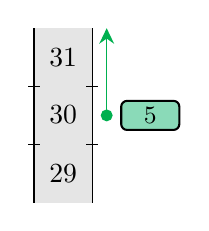
\begin{tikzpicture}[x=0.75pt,y=0.75pt,yscale=-0.7,xscale=0.7]
%uncomment if require: \path (0,300); %set diagram left start at 0, and has height of 300

%Shape: Rectangle [id:dp13563874266693043] 
\draw  [draw opacity=0][fill={rgb, 255:red, 0; green, 0; blue, 0 }  ,fill opacity=0.1 ] (230,60) -- (270,60) -- (270,180) -- (230,180) -- cycle ;
%Rounded Rect [id:dp5561959472232012] 
\draw  [fill={rgb, 255:red, 138; green, 218; blue, 184 }  ,fill opacity=1 ][line width=0.75]  (290,114) .. controls (290,111.79) and (291.79,110) .. (294,110) -- (326,110) .. controls (328.21,110) and (330,111.79) .. (330,114) -- (330,126) .. controls (330,128.21) and (328.21,130) .. (326,130) -- (294,130) .. controls (291.79,130) and (290,128.21) .. (290,126) -- cycle ;
%Straight Lines [id:da05571726881476602] 
\draw    (230,60) -- (230,180) (234,100) -- (226,100)(234,140) -- (226,140) ;
%Straight Lines [id:da7319727700794608] 
\draw    (270,60) -- (270,180) (274,100) -- (266,100)(274,140) -- (266,140) ;
%Straight Lines [id:da8116302583311774] 
\draw [color={rgb, 255:red, 0; green, 176; blue, 79 }  ,draw opacity=1 ]   (280,120) -- (280,63) ;
\draw [shift={(280,60)}, rotate = 90] [fill={rgb, 255:red, 0; green, 176; blue, 79 }  ,fill opacity=1 ][line width=0.08]  [draw opacity=0] (10.72,-5.15) -- (0,0) -- (10.72,5.15) -- (7.12,0) -- cycle    ;
\draw [shift={(280,120)}, rotate = 270] [color={rgb, 255:red, 0; green, 176; blue, 79 }  ,draw opacity=1 ][fill={rgb, 255:red, 0; green, 176; blue, 79 }  ,fill opacity=1 ][line width=0.75]      (0, 0) circle [x radius= 3.35, y radius= 3.35]   ;

% Text Node
\draw (250,80) node    {$31$};
% Text Node
\draw (250,119.5) node    {$30$};
% Text Node
\draw (310,120) node  [font=\small]  {${\textstyle 5}$};
% Text Node
\draw (250,160) node    {$29$};


\end{tikzpicture}

  \end{center}
\end{frame}

\begin{frame}{Orderbook}
  By submitting this order, Alice authorizes the exchange to accept trades on her behalf, 
  until 5 AAPL shares have been sold. Once this happens, the order is considered \textbf{filled}.

  \begin{sqt:definition}
    The exchange keeps track of each participant's \textbf{open orders} (unfilled),\\
    and collects them into an \textbf{orderbook}.
  \end{sqt:definition}

  \begin{center}
    

\tikzset{every picture/.style={line width=0.75pt}} %set default line width to 0.75pt        

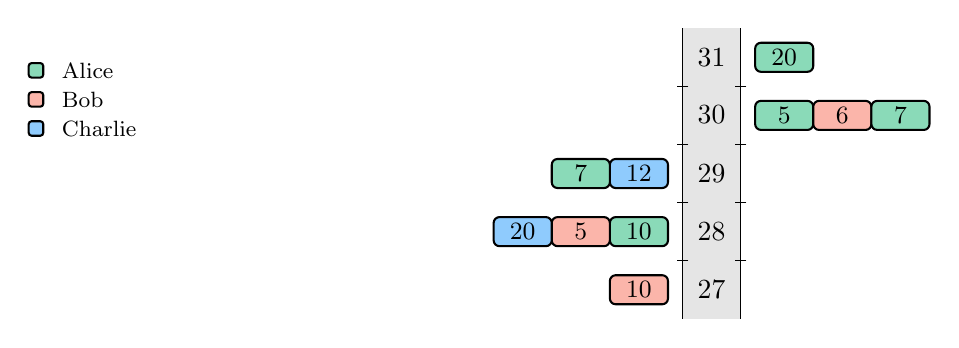
\begin{tikzpicture}[x=0.75pt,y=0.75pt,yscale=-0.7,xscale=0.7]
%%uncomment if require: \path (0,300); %set diagram left start at 0, and has height of 300

%Shape: Rectangle [id:dp8091118426371228] 
\draw  [draw opacity=0][fill={rgb, 255:red, 0; green, 0; blue, 0 }  ,fill opacity=0.1 ] (480,70) -- (520,70) -- (520,270) -- (480,270) -- cycle ;
%Rounded Rect [id:dp03190620142202172] 
\draw  [fill={rgb, 255:red, 138; green, 218; blue, 184 }  ,fill opacity=1 ][line width=0.75]  (530,124) .. controls (530,121.79) and (531.79,120) .. (534,120) -- (566,120) .. controls (568.21,120) and (570,121.79) .. (570,124) -- (570,136) .. controls (570,138.21) and (568.21,140) .. (566,140) -- (534,140) .. controls (531.79,140) and (530,138.21) .. (530,136) -- cycle ;
%Straight Lines [id:da22911621952375028] 
\draw    (480,70) -- (480,270) (484,110) -- (476,110)(484,150) -- (476,150)(484,190) -- (476,190)(484,230) -- (476,230) ;
%Straight Lines [id:da555722728776089] 
\draw    (520,70) -- (520,270) (524,110) -- (516,110)(524,150) -- (516,150)(524,190) -- (516,190)(524,230) -- (516,230) ;
%Rounded Rect [id:dp04327399535927834] 
\draw  [fill={rgb, 255:red, 251; green, 181; blue, 170 }  ,fill opacity=1 ][line width=0.75]  (570,124) .. controls (570,121.79) and (571.79,120) .. (574,120) -- (606,120) .. controls (608.21,120) and (610,121.79) .. (610,124) -- (610,136) .. controls (610,138.21) and (608.21,140) .. (606,140) -- (574,140) .. controls (571.79,140) and (570,138.21) .. (570,136) -- cycle ;
%Rounded Rect [id:dp8469096370209764] 
\draw  [fill={rgb, 255:red, 138; green, 218; blue, 184 }  ,fill opacity=1 ][line width=0.75]  (610,124) .. controls (610,121.79) and (611.79,120) .. (614,120) -- (646,120) .. controls (648.21,120) and (650,121.79) .. (650,124) -- (650,136) .. controls (650,138.21) and (648.21,140) .. (646,140) -- (614,140) .. controls (611.79,140) and (610,138.21) .. (610,136) -- cycle ;
%Rounded Rect [id:dp9977116236845125] 
\draw  [fill={rgb, 255:red, 138; green, 218; blue, 184 }  ,fill opacity=1 ][line width=0.75]  (530,84) .. controls (530,81.79) and (531.79,80) .. (534,80) -- (566,80) .. controls (568.21,80) and (570,81.79) .. (570,84) -- (570,96) .. controls (570,98.21) and (568.21,100) .. (566,100) -- (534,100) .. controls (531.79,100) and (530,98.21) .. (530,96) -- cycle ;
%Rounded Rect [id:dp40669282343922186] 
\draw  [fill={rgb, 255:red, 138; green, 218; blue, 184 }  ,fill opacity=1 ][line width=0.75]  (430,204) .. controls (430,201.79) and (431.79,200) .. (434,200) -- (466,200) .. controls (468.21,200) and (470,201.79) .. (470,204) -- (470,216) .. controls (470,218.21) and (468.21,220) .. (466,220) -- (434,220) .. controls (431.79,220) and (430,218.21) .. (430,216) -- cycle ;
%Rounded Rect [id:dp9142536483866215] 
\draw  [fill={rgb, 255:red, 143; green, 203; blue, 253 }  ,fill opacity=1 ][line width=0.75]  (430,164) .. controls (430,161.79) and (431.79,160) .. (434,160) -- (466,160) .. controls (468.21,160) and (470,161.79) .. (470,164) -- (470,176) .. controls (470,178.21) and (468.21,180) .. (466,180) -- (434,180) .. controls (431.79,180) and (430,178.21) .. (430,176) -- cycle ;
%Rounded Rect [id:dp9348427490425627] 
\draw  [fill={rgb, 255:red, 138; green, 218; blue, 184 }  ,fill opacity=1 ][line width=0.75]  (390,164) .. controls (390,161.79) and (391.79,160) .. (394,160) -- (426,160) .. controls (428.21,160) and (430,161.79) .. (430,164) -- (430,176) .. controls (430,178.21) and (428.21,180) .. (426,180) -- (394,180) .. controls (391.79,180) and (390,178.21) .. (390,176) -- cycle ;
%Rounded Rect [id:dp2667271005175228] 
\draw  [fill={rgb, 255:red, 251; green, 181; blue, 170 }  ,fill opacity=1 ][line width=0.75]  (390,204) .. controls (390,201.79) and (391.79,200) .. (394,200) -- (426,200) .. controls (428.21,200) and (430,201.79) .. (430,204) -- (430,216) .. controls (430,218.21) and (428.21,220) .. (426,220) -- (394,220) .. controls (391.79,220) and (390,218.21) .. (390,216) -- cycle ;
%Rounded Rect [id:dp5911982178413685] 
\draw  [fill={rgb, 255:red, 143; green, 203; blue, 253 }  ,fill opacity=1 ][line width=0.75]  (350,204) .. controls (350,201.79) and (351.79,200) .. (354,200) -- (386,200) .. controls (388.21,200) and (390,201.79) .. (390,204) -- (390,216) .. controls (390,218.21) and (388.21,220) .. (386,220) -- (354,220) .. controls (351.79,220) and (350,218.21) .. (350,216) -- cycle ;
%Rounded Rect [id:dp9977666228162302] 
\draw  [fill={rgb, 255:red, 251; green, 181; blue, 170 }  ,fill opacity=1 ][line width=0.75]  (430,244) .. controls (430,241.79) and (431.79,240) .. (434,240) -- (466,240) .. controls (468.21,240) and (470,241.79) .. (470,244) -- (470,256) .. controls (470,258.21) and (468.21,260) .. (466,260) -- (434,260) .. controls (431.79,260) and (430,258.21) .. (430,256) -- cycle ;
%Rounded Rect [id:dp0318183239720361] 
\draw  [fill={rgb, 255:red, 138; green, 218; blue, 184 }  ,fill opacity=1 ][line width=0.75]  (30,96) .. controls (30,94.9) and (30.9,94) .. (32,94) -- (38,94) .. controls (39.1,94) and (40,94.9) .. (40,96) -- (40,102) .. controls (40,103.1) and (39.1,104) .. (38,104) -- (32,104) .. controls (30.9,104) and (30,103.1) .. (30,102) -- cycle ;
%Rounded Rect [id:dp16680821822273184] 
\draw  [fill={rgb, 255:red, 143; green, 203; blue, 253 }  ,fill opacity=1 ][line width=0.75]  (30,136) .. controls (30,134.9) and (30.9,134) .. (32,134) -- (38,134) .. controls (39.1,134) and (40,134.9) .. (40,136) -- (40,142) .. controls (40,143.1) and (39.1,144) .. (38,144) -- (32,144) .. controls (30.9,144) and (30,143.1) .. (30,142) -- cycle ;
%Rounded Rect [id:dp4425250472328628] 
\draw  [fill={rgb, 255:red, 251; green, 181; blue, 170 }  ,fill opacity=1 ][line width=0.75]  (30,116) .. controls (30,114.9) and (30.9,114) .. (32,114) -- (38,114) .. controls (39.1,114) and (40,114.9) .. (40,116) -- (40,122) .. controls (40,123.1) and (39.1,124) .. (38,124) -- (32,124) .. controls (30.9,124) and (30,123.1) .. (30,122) -- cycle ;

% Text Node
\draw (500,90) node    {$31$};
% Text Node
\draw (500,129.5) node    {$30$};
% Text Node
\draw (550,130) node  [font=\small]  {${\textstyle 5}$};
% Text Node
\draw (500,170) node    {$29$};
% Text Node
\draw (500,210) node    {$28$};
% Text Node
\draw (500,250) node    {$27$};
% Text Node
\draw (590,130) node  [font=\small]  {$6$};
% Text Node
\draw (630,130) node  [font=\small]  {$7$};
% Text Node
\draw (550,90) node  [font=\small]  {$20$};
% Text Node
\draw (450,210) node  [font=\small]  {$10$};
% Text Node
\draw (450,170) node  [font=\small]  {$12$};
% Text Node
\draw (410,170) node  [font=\small]  {$7$};
% Text Node
\draw (410,210) node  [font=\small]  {${\textstyle 5}$};
% Text Node
\draw (370,210) node  [font=\small]  {$20$};
% Text Node
\draw (450,250) node  [font=\small]  {$10$};
% Text Node
\draw (51,92) node [anchor=north west][inner sep=0.75pt]  [font=\footnotesize] [align=left] {Alice};
% Text Node
\draw (51,112) node [anchor=north west][inner sep=0.75pt]  [font=\footnotesize] [align=left] {Bob};
% Text Node
\draw (51,132) node [anchor=north west][inner sep=0.75pt]  [font=\footnotesize] [align=left] {Charlie};


\end{tikzpicture}

  \end{center}
\end{frame}

\begin{frame}{Limit Orders In Cross}

  \begin{sqt:definition}
    Two limit orders are \textbf{in cross} if
    \begin{itemize}
      \item One order is a \textbf{bid} and the other is an \textbf{ask}.
      \item There exists an \textbf{intersection} between the price ranges they are willing to trade at
    \end{itemize}
  \end{sqt:definition}
\end{frame}

\section{Order Matching}

\begin{frame}{Order Matching Algorithm}
  We will demonstrate \textbf{continuous matching} with \textbf{price-time priority}.\\
  This is a \textbf{matching algorithm} that determines the trades made when orders are inserted.

  \begin{itemize}
    \item Orders are \textbf{received} and then \textbf{handled} by the exchange one at a time.
    \item The order currently being \textbf{handled} is the \textbf{aggressing order}.
    \item The \textbf{aggressing order} is matched against \textbf{open orders} it is \textbf{in cross} with.
    \begin{itemize}
      \item Choose the \textbf{open order} according to \textbf{price-time priority}.
      \item Execute the trade at the price level of the \textbf{open order}, for the maximum quantity possible.
    \end{itemize}
    \item This matching occurs until either:
    \begin{itemize}
      \item The aggressing order runs out of quantity:
      \begin{itemize}
        \item The order is considered \textbf{filled} and is discarded.
      \end{itemize}
      \item No more orders \textbf{in cross} remain:
      \begin{itemize}
        \item The order is \textbf{unfilled} or only \textbf{partially filled}.
        \item If the order was a \textbf{fill-and-kill} (FAK), then the order is discarded.
        \item If the order was a \textbf{good-till-cancel} (GTC), then it is inserted at its price level at the back of the queue.
      \end{itemize}
    \end{itemize}
  \end{itemize}
\end{frame}

\begin{frame}{Small GTC Buy Order: Initial}
  \begin{center}
    \input{assets/small_gtc_frame_0.tex}
  \end{center}
\end{frame}

\begin{frame}{Small GTC Buy Order: Animation}
  \begin{center}
    \only<1>{\input{assets/small_gtc_frame_1.tex}}
    \only<2>{\input{assets/small_gtc_frame_2.tex}}
    \only<3>{

\tikzset{every picture/.style={line width=0.75pt}} %set default line width to 0.75pt        

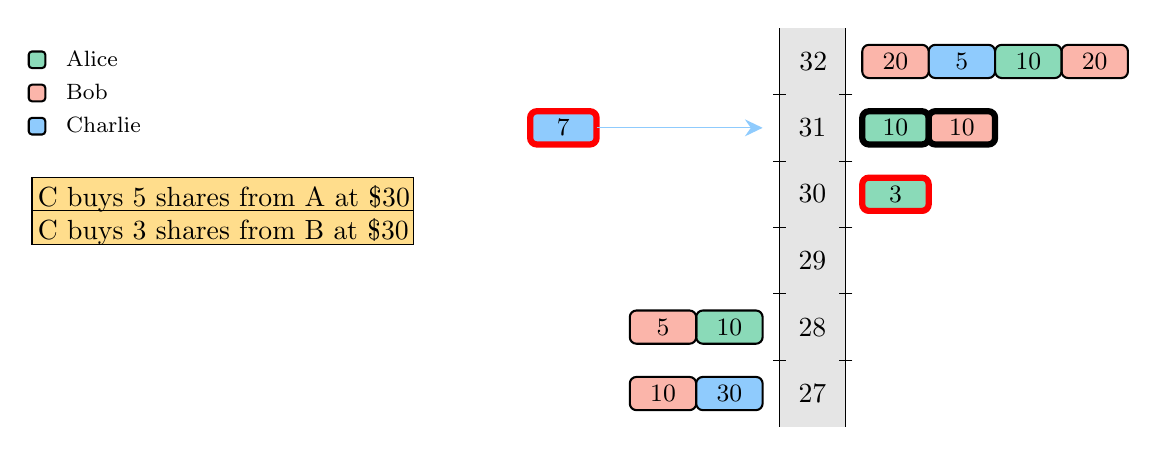
\begin{tikzpicture}[x=0.75pt,y=0.75pt,yscale=-0.8,xscale=0.8]
%uncomment if require: \path (0,300); %set diagram left start at 0, and has height of 300


%Shape: Rectangle [id:dp0819038861204413] 
\draw  [draw opacity=0][fill={rgb, 255:red, 0; green, 0; blue, 0 }  ,fill opacity=0.1 ] (480,30) -- (520,30) -- (520,270) -- (480,270) -- cycle ;
%Straight Lines [id:da11910476519653257] 
\draw    (480,30) -- (480,270) (484,70) -- (476,70)(484,110) -- (476,110)(484,150) -- (476,150)(484,190) -- (476,190)(484,230) -- (476,230) ;
%Straight Lines [id:da6345525229446171] 
\draw    (520,30) -- (520,270) (524,70) -- (516,70)(524,110) -- (516,110)(524,150) -- (516,150)(524,190) -- (516,190)(524,230) -- (516,230) ;
%Rounded Rect [id:dp5841732804090376] 
\draw  [color={rgb, 255:red, 255; green, 0; blue, 0 }  ,draw opacity=1 ][fill={rgb, 255:red, 138; green, 218; blue, 184 }  ,fill opacity=1 ][line width=2.25]  (530,124) .. controls (530,121.79) and (531.79,120) .. (534,120) -- (566,120) .. controls (568.21,120) and (570,121.79) .. (570,124) -- (570,136) .. controls (570,138.21) and (568.21,140) .. (566,140) -- (534,140) .. controls (531.79,140) and (530,138.21) .. (530,136) -- cycle ;
%Rounded Rect [id:dp1834680548544293] 
\draw  [color={rgb, 255:red, 0; green, 0; blue, 0 }  ,draw opacity=1 ][fill={rgb, 255:red, 138; green, 218; blue, 184 }  ,fill opacity=1 ][line width=2.25]  (530,84) .. controls (530,81.79) and (531.79,80) .. (534,80) -- (566,80) .. controls (568.21,80) and (570,81.79) .. (570,84) -- (570,96) .. controls (570,98.21) and (568.21,100) .. (566,100) -- (534,100) .. controls (531.79,100) and (530,98.21) .. (530,96) -- cycle ;
%Rounded Rect [id:dp9540702911156453] 
\draw  [fill={rgb, 255:red, 138; green, 218; blue, 184 }  ,fill opacity=1 ][line width=0.75]  (430,204) .. controls (430,201.79) and (431.79,200) .. (434,200) -- (466,200) .. controls (468.21,200) and (470,201.79) .. (470,204) -- (470,216) .. controls (470,218.21) and (468.21,220) .. (466,220) -- (434,220) .. controls (431.79,220) and (430,218.21) .. (430,216) -- cycle ;
%Rounded Rect [id:dp11917240068278401] 
\draw  [fill={rgb, 255:red, 251; green, 181; blue, 170 }  ,fill opacity=1 ][line width=0.75]  (390,204) .. controls (390,201.79) and (391.79,200) .. (394,200) -- (426,200) .. controls (428.21,200) and (430,201.79) .. (430,204) -- (430,216) .. controls (430,218.21) and (428.21,220) .. (426,220) -- (394,220) .. controls (391.79,220) and (390,218.21) .. (390,216) -- cycle ;
%Rounded Rect [id:dp7245467196534818] 
\draw  [fill={rgb, 255:red, 251; green, 181; blue, 170 }  ,fill opacity=1 ][line width=0.75]  (390,244) .. controls (390,241.79) and (391.79,240) .. (394,240) -- (426,240) .. controls (428.21,240) and (430,241.79) .. (430,244) -- (430,256) .. controls (430,258.21) and (428.21,260) .. (426,260) -- (394,260) .. controls (391.79,260) and (390,258.21) .. (390,256) -- cycle ;
%Rounded Rect [id:dp03827927607995818] 
\draw  [fill={rgb, 255:red, 138; green, 218; blue, 184 }  ,fill opacity=1 ][line width=0.75]  (28,46) .. controls (28,44.9) and (28.9,44) .. (30,44) -- (36,44) .. controls (37.1,44) and (38,44.9) .. (38,46) -- (38,52) .. controls (38,53.1) and (37.1,54) .. (36,54) -- (30,54) .. controls (28.9,54) and (28,53.1) .. (28,52) -- cycle ;
%Rounded Rect [id:dp7222729266059345] 
\draw  [fill={rgb, 255:red, 143; green, 203; blue, 253 }  ,fill opacity=1 ][line width=0.75]  (28,86) .. controls (28,84.9) and (28.9,84) .. (30,84) -- (36,84) .. controls (37.1,84) and (38,84.9) .. (38,86) -- (38,92) .. controls (38,93.1) and (37.1,94) .. (36,94) -- (30,94) .. controls (28.9,94) and (28,93.1) .. (28,92) -- cycle ;
%Rounded Rect [id:dp3636132794332668] 
\draw  [fill={rgb, 255:red, 251; green, 181; blue, 170 }  ,fill opacity=1 ][line width=0.75]  (28,66) .. controls (28,64.9) and (28.9,64) .. (30,64) -- (36,64) .. controls (37.1,64) and (38,64.9) .. (38,66) -- (38,72) .. controls (38,73.1) and (37.1,74) .. (36,74) -- (30,74) .. controls (28.9,74) and (28,73.1) .. (28,72) -- cycle ;
%Rounded Rect [id:dp46209137558796687] 
\draw  [color={rgb, 255:red, 0; green, 0; blue, 0 }  ,draw opacity=1 ][fill={rgb, 255:red, 251; green, 181; blue, 170 }  ,fill opacity=1 ][line width=2.25]  (570,84) .. controls (570,81.79) and (571.79,80) .. (574,80) -- (606,80) .. controls (608.21,80) and (610,81.79) .. (610,84) -- (610,96) .. controls (610,98.21) and (608.21,100) .. (606,100) -- (574,100) .. controls (571.79,100) and (570,98.21) .. (570,96) -- cycle ;
%Rounded Rect [id:dp866142470002609] 
\draw  [fill={rgb, 255:red, 143; green, 203; blue, 253 }  ,fill opacity=1 ][line width=0.75]  (570,44) .. controls (570,41.79) and (571.79,40) .. (574,40) -- (606,40) .. controls (608.21,40) and (610,41.79) .. (610,44) -- (610,56) .. controls (610,58.21) and (608.21,60) .. (606,60) -- (574,60) .. controls (571.79,60) and (570,58.21) .. (570,56) -- cycle ;
%Rounded Rect [id:dp708981159795911] 
\draw  [fill={rgb, 255:red, 143; green, 203; blue, 253 }  ,fill opacity=1 ][line width=0.75]  (430,244) .. controls (430,241.79) and (431.79,240) .. (434,240) -- (466,240) .. controls (468.21,240) and (470,241.79) .. (470,244) -- (470,256) .. controls (470,258.21) and (468.21,260) .. (466,260) -- (434,260) .. controls (431.79,260) and (430,258.21) .. (430,256) -- cycle ;
%Rounded Rect [id:dp7591462434368331] 
\draw  [color={rgb, 255:red, 255; green, 0; blue, 0 }  ,draw opacity=1 ][fill={rgb, 255:red, 143; green, 203; blue, 253 }  ,fill opacity=1 ][line width=2.25]  (330,84) .. controls (330,81.79) and (331.79,80) .. (334,80) -- (366,80) .. controls (368.21,80) and (370,81.79) .. (370,84) -- (370,96) .. controls (370,98.21) and (368.21,100) .. (366,100) -- (334,100) .. controls (331.79,100) and (330,98.21) .. (330,96) -- cycle ;
%Straight Lines [id:da013136060541545924] 
\draw [color={rgb, 255:red, 143; green, 203; blue, 253 }  ,draw opacity=1 ]   (370,90) -- (467,90) ;
\draw [shift={(470,90)}, rotate = 180] [fill={rgb, 255:red, 143; green, 203; blue, 253 }  ,fill opacity=1 ][line width=0.08]  [draw opacity=0] (10.72,-5.15) -- (0,0) -- (10.72,5.15) -- (7.12,0) -- cycle    ;
%Rounded Rect [id:dp0037524200066810787] 
\draw  [fill={rgb, 255:red, 251; green, 181; blue, 170 }  ,fill opacity=1 ][line width=0.75]  (530,44) .. controls (530,41.79) and (531.79,40) .. (534,40) -- (566,40) .. controls (568.21,40) and (570,41.79) .. (570,44) -- (570,56) .. controls (570,58.21) and (568.21,60) .. (566,60) -- (534,60) .. controls (531.79,60) and (530,58.21) .. (530,56) -- cycle ;
%Rounded Rect [id:dp15509522152906374] 
\draw  [fill={rgb, 255:red, 251; green, 181; blue, 170 }  ,fill opacity=1 ][line width=0.75]  (650,44) .. controls (650,41.79) and (651.79,40) .. (654,40) -- (686,40) .. controls (688.21,40) and (690,41.79) .. (690,44) -- (690,56) .. controls (690,58.21) and (688.21,60) .. (686,60) -- (654,60) .. controls (651.79,60) and (650,58.21) .. (650,56) -- cycle ;
%Rounded Rect [id:dp31347310397506256] 
\draw  [fill={rgb, 255:red, 138; green, 218; blue, 184 }  ,fill opacity=1 ][line width=0.75]  (610,44) .. controls (610,41.79) and (611.79,40) .. (614,40) -- (646,40) .. controls (648.21,40) and (650,41.79) .. (650,44) -- (650,56) .. controls (650,58.21) and (648.21,60) .. (646,60) -- (614,60) .. controls (611.79,60) and (610,58.21) .. (610,56) -- cycle ;
%Shape: Rectangle [id:dp14290409086582512] 
\draw  [fill={rgb, 255:red, 255; green, 221; blue, 140 }  ,fill opacity=1 ] (30,120) -- (260,120) -- (260,140) -- (30,140) -- cycle ;
%Shape: Rectangle [id:dp6436928446902445] 
\draw  [fill={rgb, 255:red, 255; green, 221; blue, 140 }  ,fill opacity=1 ] (30,140) -- (260,140) -- (260,160) -- (30,160) -- cycle ;

% Text Node
\draw (500,90) node    {$31$};
% Text Node
\draw (500,129.5) node    {$30$};
% Text Node
\draw (500,170) node    {$29$};
% Text Node
\draw (500,210) node    {$28$};
% Text Node
\draw (500,250) node    {$27$};
% Text Node
\draw (550,130) node  [font=\small]  {$3$};
% Text Node
\draw (550,90) node  [font=\small]  {$10$};
% Text Node
\draw (450,210) node  [font=\small]  {$10$};
% Text Node
\draw (410,210) node  [font=\small]  {${\textstyle 5}$};
% Text Node
\draw (410,250) node  [font=\small]  {$10$};
% Text Node
\draw (49,42) node [anchor=north west][inner sep=0.75pt]  [font=\footnotesize] [align=left] {Alice};
% Text Node
\draw (49,62) node [anchor=north west][inner sep=0.75pt]  [font=\footnotesize] [align=left] {Bob};
% Text Node
\draw (49,82) node [anchor=north west][inner sep=0.75pt]  [font=\footnotesize] [align=left] {Charlie};
% Text Node
\draw (590,90) node  [font=\small]  {$10$};
% Text Node
\draw (500.5,50) node    {$32$};
% Text Node
\draw (590,50) node  [font=\small]  {$5$};
% Text Node
\draw (450,250) node  [font=\small]  {$30$};
% Text Node
\draw (350,90) node  [font=\small]  {$7$};
% Text Node
% Text Node
\draw (550,50) node  [font=\small]  {$20$};
% Text Node
\draw (670,50) node  [font=\small]  {$20$};
% Text Node
\draw (630,50) node  [font=\small]  {$10$};
% Text Node
\draw (32,123) node [anchor=north west][inner sep=0.75pt]   [align=left] {C buys 5 shares from A at \$30};
% Text Node
\draw (32,143) node [anchor=north west][inner sep=0.75pt]   [align=left] {C buys 3 shares from B at \$30};


\end{tikzpicture}
}
    \only<4>{\input{assets/small_gtc_frame_4.tex}}
    \only<5>{\input{assets/small_gtc_frame_5.tex}}
  \end{center}
\end{frame}

\begin{frame}{Small GTC Buy Order: Result}
  \begin{center}
    \input{assets/small_gtc_frame_result.tex}
  \end{center}
\end{frame}

\begin{frame}{Large GTC Buy Order: Initial}
  \begin{center}
    \input{assets/large_gtc_frame_0.tex}
  \end{center}
\end{frame}

\begin{frame}{Large GTC Buy Order: Animation}
  \begin{center}
    \only<1>{\input{assets/large_gtc_frame_1.tex}}
    \only<2>{\input{assets/large_gtc_frame_2.tex}}
    \only<3>{\input{assets/large_gtc_frame_3.tex}}
    \only<4>{\input{assets/large_gtc_frame_4.tex}}
    \only<5>{

\tikzset{every picture/.style={line width=0.75pt}} %set default line width to 0.75pt        

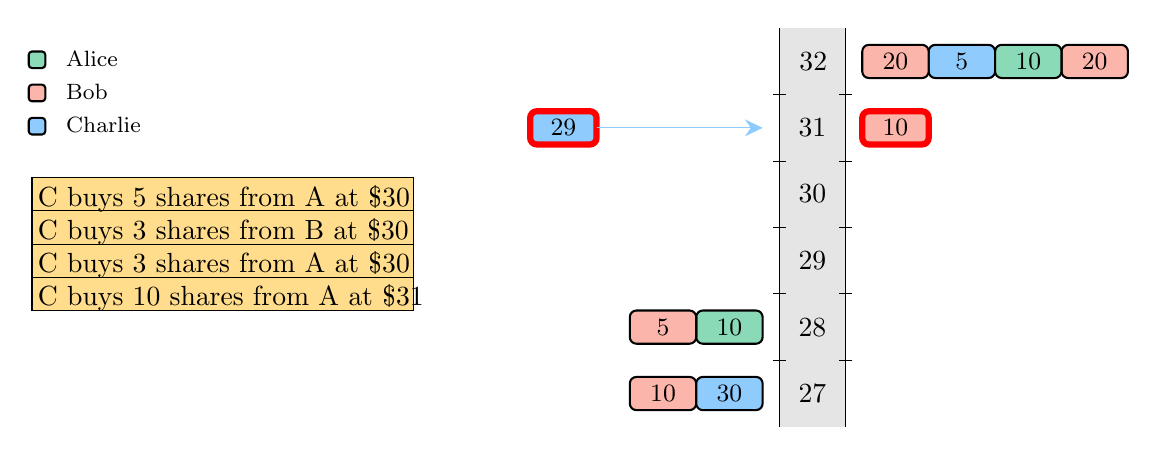
\begin{tikzpicture}[x=0.75pt,y=0.75pt,yscale=-0.8,xscale=0.8]
%uncomment if require: \path (0,300); %set diagram left start at 0, and has height of 300


%Shape: Rectangle [id:dp8337814582471778] 
\draw  [draw opacity=0][fill={rgb, 255:red, 0; green, 0; blue, 0 }  ,fill opacity=0.1 ] (470,40) -- (510,40) -- (510,280) -- (470,280) -- cycle ;
%Straight Lines [id:da09969873094924853] 
\draw    (470,40) -- (470,280) (474,80) -- (466,80)(474,120) -- (466,120)(474,160) -- (466,160)(474,200) -- (466,200)(474,240) -- (466,240) ;
%Straight Lines [id:da5936664441336669] 
\draw    (510,40) -- (510,280) (514,80) -- (506,80)(514,120) -- (506,120)(514,160) -- (506,160)(514,200) -- (506,200)(514,240) -- (506,240) ;
%Rounded Rect [id:dp21774022020109518] 
\draw  [fill={rgb, 255:red, 138; green, 218; blue, 184 }  ,fill opacity=1 ][line width=0.75]  (420,214) .. controls (420,211.79) and (421.79,210) .. (424,210) -- (456,210) .. controls (458.21,210) and (460,211.79) .. (460,214) -- (460,226) .. controls (460,228.21) and (458.21,230) .. (456,230) -- (424,230) .. controls (421.79,230) and (420,228.21) .. (420,226) -- cycle ;
%Rounded Rect [id:dp27872897957842435] 
\draw  [fill={rgb, 255:red, 251; green, 181; blue, 170 }  ,fill opacity=1 ][line width=0.75]  (380,214) .. controls (380,211.79) and (381.79,210) .. (384,210) -- (416,210) .. controls (418.21,210) and (420,211.79) .. (420,214) -- (420,226) .. controls (420,228.21) and (418.21,230) .. (416,230) -- (384,230) .. controls (381.79,230) and (380,228.21) .. (380,226) -- cycle ;
%Rounded Rect [id:dp2087008923376935] 
\draw  [fill={rgb, 255:red, 251; green, 181; blue, 170 }  ,fill opacity=1 ][line width=0.75]  (380,254) .. controls (380,251.79) and (381.79,250) .. (384,250) -- (416,250) .. controls (418.21,250) and (420,251.79) .. (420,254) -- (420,266) .. controls (420,268.21) and (418.21,270) .. (416,270) -- (384,270) .. controls (381.79,270) and (380,268.21) .. (380,266) -- cycle ;
%Rounded Rect [id:dp1281757847349283] 
\draw  [fill={rgb, 255:red, 138; green, 218; blue, 184 }  ,fill opacity=1 ][line width=0.75]  (18,56) .. controls (18,54.9) and (18.9,54) .. (20,54) -- (26,54) .. controls (27.1,54) and (28,54.9) .. (28,56) -- (28,62) .. controls (28,63.1) and (27.1,64) .. (26,64) -- (20,64) .. controls (18.9,64) and (18,63.1) .. (18,62) -- cycle ;
%Rounded Rect [id:dp9520385717692255] 
\draw  [fill={rgb, 255:red, 143; green, 203; blue, 253 }  ,fill opacity=1 ][line width=0.75]  (18,96) .. controls (18,94.9) and (18.9,94) .. (20,94) -- (26,94) .. controls (27.1,94) and (28,94.9) .. (28,96) -- (28,102) .. controls (28,103.1) and (27.1,104) .. (26,104) -- (20,104) .. controls (18.9,104) and (18,103.1) .. (18,102) -- cycle ;
%Rounded Rect [id:dp4915947371569024] 
\draw  [fill={rgb, 255:red, 251; green, 181; blue, 170 }  ,fill opacity=1 ][line width=0.75]  (18,76) .. controls (18,74.9) and (18.9,74) .. (20,74) -- (26,74) .. controls (27.1,74) and (28,74.9) .. (28,76) -- (28,82) .. controls (28,83.1) and (27.1,84) .. (26,84) -- (20,84) .. controls (18.9,84) and (18,83.1) .. (18,82) -- cycle ;
%Rounded Rect [id:dp1657885524180357] 
\draw  [color={rgb, 255:red, 255; green, 0; blue, 0 }  ,draw opacity=1 ][fill={rgb, 255:red, 251; green, 181; blue, 170 }  ,fill opacity=1 ][line width=2.25]  (520,94) .. controls (520,91.79) and (521.79,90) .. (524,90) -- (556,90) .. controls (558.21,90) and (560,91.79) .. (560,94) -- (560,106) .. controls (560,108.21) and (558.21,110) .. (556,110) -- (524,110) .. controls (521.79,110) and (520,108.21) .. (520,106) -- cycle ;
%Rounded Rect [id:dp19440278883646667] 
\draw  [fill={rgb, 255:red, 143; green, 203; blue, 253 }  ,fill opacity=1 ][line width=0.75]  (560,54) .. controls (560,51.79) and (561.79,50) .. (564,50) -- (596,50) .. controls (598.21,50) and (600,51.79) .. (600,54) -- (600,66) .. controls (600,68.21) and (598.21,70) .. (596,70) -- (564,70) .. controls (561.79,70) and (560,68.21) .. (560,66) -- cycle ;
%Rounded Rect [id:dp11444604878691622] 
\draw  [fill={rgb, 255:red, 143; green, 203; blue, 253 }  ,fill opacity=1 ][line width=0.75]  (420,254) .. controls (420,251.79) and (421.79,250) .. (424,250) -- (456,250) .. controls (458.21,250) and (460,251.79) .. (460,254) -- (460,266) .. controls (460,268.21) and (458.21,270) .. (456,270) -- (424,270) .. controls (421.79,270) and (420,268.21) .. (420,266) -- cycle ;
%Rounded Rect [id:dp6379504097709302] 
\draw  [color={rgb, 255:red, 255; green, 0; blue, 0 }  ,draw opacity=1 ][fill={rgb, 255:red, 143; green, 203; blue, 253 }  ,fill opacity=1 ][line width=2.25]  (320,94) .. controls (320,91.79) and (321.79,90) .. (324,90) -- (356,90) .. controls (358.21,90) and (360,91.79) .. (360,94) -- (360,106) .. controls (360,108.21) and (358.21,110) .. (356,110) -- (324,110) .. controls (321.79,110) and (320,108.21) .. (320,106) -- cycle ;
%Straight Lines [id:da5639250481518682] 
\draw [color={rgb, 255:red, 143; green, 203; blue, 253 }  ,draw opacity=1 ]   (360,100) -- (457,100) ;
\draw [shift={(460,100)}, rotate = 180] [fill={rgb, 255:red, 143; green, 203; blue, 253 }  ,fill opacity=1 ][line width=0.08]  [draw opacity=0] (10.72,-5.15) -- (0,0) -- (10.72,5.15) -- (7.12,0) -- cycle    ;
%Rounded Rect [id:dp7706984934543188] 
\draw  [fill={rgb, 255:red, 251; green, 181; blue, 170 }  ,fill opacity=1 ][line width=0.75]  (520,54) .. controls (520,51.79) and (521.79,50) .. (524,50) -- (556,50) .. controls (558.21,50) and (560,51.79) .. (560,54) -- (560,66) .. controls (560,68.21) and (558.21,70) .. (556,70) -- (524,70) .. controls (521.79,70) and (520,68.21) .. (520,66) -- cycle ;
%Rounded Rect [id:dp49004438558198016] 
\draw  [fill={rgb, 255:red, 251; green, 181; blue, 170 }  ,fill opacity=1 ][line width=0.75]  (640,54) .. controls (640,51.79) and (641.79,50) .. (644,50) -- (676,50) .. controls (678.21,50) and (680,51.79) .. (680,54) -- (680,66) .. controls (680,68.21) and (678.21,70) .. (676,70) -- (644,70) .. controls (641.79,70) and (640,68.21) .. (640,66) -- cycle ;
%Rounded Rect [id:dp17939821006978351] 
\draw  [fill={rgb, 255:red, 138; green, 218; blue, 184 }  ,fill opacity=1 ][line width=0.75]  (600,54) .. controls (600,51.79) and (601.79,50) .. (604,50) -- (636,50) .. controls (638.21,50) and (640,51.79) .. (640,54) -- (640,66) .. controls (640,68.21) and (638.21,70) .. (636,70) -- (604,70) .. controls (601.79,70) and (600,68.21) .. (600,66) -- cycle ;
%Shape: Rectangle [id:dp9403473417630838] 
\draw  [fill={rgb, 255:red, 255; green, 221; blue, 140 }  ,fill opacity=1 ] (20,130) -- (250,130) -- (250,150) -- (20,150) -- cycle ;
%Shape: Rectangle [id:dp49072857961828886] 
\draw  [fill={rgb, 255:red, 255; green, 221; blue, 140 }  ,fill opacity=1 ] (20,150) -- (250,150) -- (250,170) -- (20,170) -- cycle ;
%Shape: Rectangle [id:dp9961567428739467] 
\draw  [fill={rgb, 255:red, 255; green, 221; blue, 140 }  ,fill opacity=1 ] (20,190) -- (250,190) -- (250,210) -- (20,210) -- cycle ;
%Shape: Rectangle [id:dp3060916994428581] 
\draw  [fill={rgb, 255:red, 255; green, 221; blue, 140 }  ,fill opacity=1 ] (20,170) -- (250,170) -- (250,190) -- (20,190) -- cycle ;

% Text Node
\draw (490,100) node    {$31$};
% Text Node
\draw (490,139.5) node    {$30$};
% Text Node
\draw (490,180) node    {$29$};
% Text Node
\draw (490,220) node    {$28$};
% Text Node
\draw (490,260) node    {$27$};
% Text Node
\draw (440,220) node  [font=\small]  {$10$};
% Text Node
\draw (400,220) node  [font=\small]  {${\textstyle 5}$};
% Text Node
\draw (400,260) node  [font=\small]  {$10$};
% Text Node
\draw (39,52) node [anchor=north west][inner sep=0.75pt]  [font=\footnotesize] [align=left] {Alice};
% Text Node
\draw (39,72) node [anchor=north west][inner sep=0.75pt]  [font=\footnotesize] [align=left] {Bob};
% Text Node
\draw (39,92) node [anchor=north west][inner sep=0.75pt]  [font=\footnotesize] [align=left] {Charlie};
% Text Node
\draw (540,100) node  [font=\small]  {$10$};
% Text Node
\draw (490.5,60) node    {$32$};
% Text Node
\draw (580,60) node  [font=\small]  {$5$};
% Text Node
\draw (440,260) node  [font=\small]  {$30$};
% Text Node
\draw (340,100) node  [font=\small]  {$29$};
% Text Node
\draw (540,60) node  [font=\small]  {$20$};
% Text Node
\draw (660,60) node  [font=\small]  {$20$};
% Text Node
\draw (620,60) node  [font=\small]  {$10$};
% Text Node
\draw (22,133) node [anchor=north west][inner sep=0.75pt]   [align=left] {C buys 5 shares from A at \$30};
% Text Node
\draw (22,153) node [anchor=north west][inner sep=0.75pt]   [align=left] {C buys 3 shares from B at \$30};
% Text Node
\draw (22,193) node [anchor=north west][inner sep=0.75pt]   [align=left] {C buys 10 shares from A at \$31};
% Text Node
\draw (22,173) node [anchor=north west][inner sep=0.75pt]   [align=left] {C buys 3 shares from A at \$30};


\end{tikzpicture}
}
    \only<6>{

\tikzset{every picture/.style={line width=0.75pt}} %set default line width to 0.75pt        

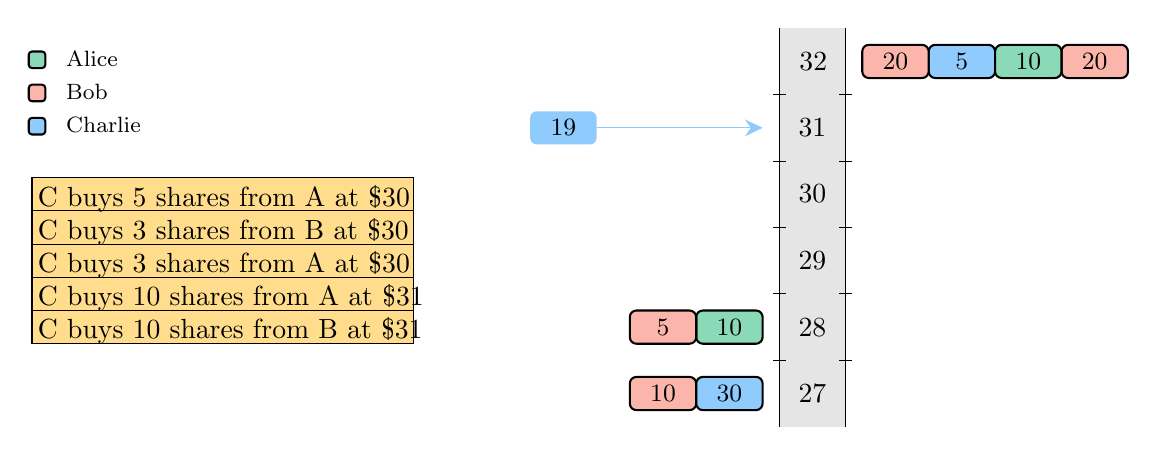
\begin{tikzpicture}[x=0.75pt,y=0.75pt,yscale=-0.8,xscale=0.8]
%uncomment if require: \path (0,300); %set diagram left start at 0, and has height of 300

%Shape: Rectangle [id:dp3861715993266832] 
\draw  [draw opacity=0][fill={rgb, 255:red, 0; green, 0; blue, 0 }  ,fill opacity=0.1 ] (470,40) -- (510,40) -- (510,280) -- (470,280) -- cycle ;
%Straight Lines [id:da8309385407681799] 
\draw    (470,40) -- (470,280) (474,80) -- (466,80)(474,120) -- (466,120)(474,160) -- (466,160)(474,200) -- (466,200)(474,240) -- (466,240) ;
%Straight Lines [id:da5801335245942738] 
\draw    (510,40) -- (510,280) (514,80) -- (506,80)(514,120) -- (506,120)(514,160) -- (506,160)(514,200) -- (506,200)(514,240) -- (506,240) ;
%Rounded Rect [id:dp937444837474773] 
\draw  [fill={rgb, 255:red, 138; green, 218; blue, 184 }  ,fill opacity=1 ][line width=0.75]  (420,214) .. controls (420,211.79) and (421.79,210) .. (424,210) -- (456,210) .. controls (458.21,210) and (460,211.79) .. (460,214) -- (460,226) .. controls (460,228.21) and (458.21,230) .. (456,230) -- (424,230) .. controls (421.79,230) and (420,228.21) .. (420,226) -- cycle ;
%Rounded Rect [id:dp6370281869352094] 
\draw  [fill={rgb, 255:red, 251; green, 181; blue, 170 }  ,fill opacity=1 ][line width=0.75]  (380,214) .. controls (380,211.79) and (381.79,210) .. (384,210) -- (416,210) .. controls (418.21,210) and (420,211.79) .. (420,214) -- (420,226) .. controls (420,228.21) and (418.21,230) .. (416,230) -- (384,230) .. controls (381.79,230) and (380,228.21) .. (380,226) -- cycle ;
%Rounded Rect [id:dp9214685747053574] 
\draw  [fill={rgb, 255:red, 251; green, 181; blue, 170 }  ,fill opacity=1 ][line width=0.75]  (380,254) .. controls (380,251.79) and (381.79,250) .. (384,250) -- (416,250) .. controls (418.21,250) and (420,251.79) .. (420,254) -- (420,266) .. controls (420,268.21) and (418.21,270) .. (416,270) -- (384,270) .. controls (381.79,270) and (380,268.21) .. (380,266) -- cycle ;
%Rounded Rect [id:dp5437621877409694] 
\draw  [fill={rgb, 255:red, 138; green, 218; blue, 184 }  ,fill opacity=1 ][line width=0.75]  (18,56) .. controls (18,54.9) and (18.9,54) .. (20,54) -- (26,54) .. controls (27.1,54) and (28,54.9) .. (28,56) -- (28,62) .. controls (28,63.1) and (27.1,64) .. (26,64) -- (20,64) .. controls (18.9,64) and (18,63.1) .. (18,62) -- cycle ;
%Rounded Rect [id:dp09068402110649876] 
\draw  [fill={rgb, 255:red, 143; green, 203; blue, 253 }  ,fill opacity=1 ][line width=0.75]  (18,96) .. controls (18,94.9) and (18.9,94) .. (20,94) -- (26,94) .. controls (27.1,94) and (28,94.9) .. (28,96) -- (28,102) .. controls (28,103.1) and (27.1,104) .. (26,104) -- (20,104) .. controls (18.9,104) and (18,103.1) .. (18,102) -- cycle ;
%Rounded Rect [id:dp6353505724561966] 
\draw  [fill={rgb, 255:red, 251; green, 181; blue, 170 }  ,fill opacity=1 ][line width=0.75]  (18,76) .. controls (18,74.9) and (18.9,74) .. (20,74) -- (26,74) .. controls (27.1,74) and (28,74.9) .. (28,76) -- (28,82) .. controls (28,83.1) and (27.1,84) .. (26,84) -- (20,84) .. controls (18.9,84) and (18,83.1) .. (18,82) -- cycle ;
%Rounded Rect [id:dp6699541273577541] 
\draw  [fill={rgb, 255:red, 143; green, 203; blue, 253 }  ,fill opacity=1 ][line width=0.75]  (560,54) .. controls (560,51.79) and (561.79,50) .. (564,50) -- (596,50) .. controls (598.21,50) and (600,51.79) .. (600,54) -- (600,66) .. controls (600,68.21) and (598.21,70) .. (596,70) -- (564,70) .. controls (561.79,70) and (560,68.21) .. (560,66) -- cycle ;
%Rounded Rect [id:dp9726118728538371] 
\draw  [fill={rgb, 255:red, 143; green, 203; blue, 253 }  ,fill opacity=1 ][line width=0.75]  (420,254) .. controls (420,251.79) and (421.79,250) .. (424,250) -- (456,250) .. controls (458.21,250) and (460,251.79) .. (460,254) -- (460,266) .. controls (460,268.21) and (458.21,270) .. (456,270) -- (424,270) .. controls (421.79,270) and (420,268.21) .. (420,266) -- cycle ;
%Rounded Rect [id:dp36723448056690344] 
\draw  [draw opacity=0][fill={rgb, 255:red, 143; green, 203; blue, 253 }  ,fill opacity=1 ][line width=2.25]  (320,94) .. controls (320,91.79) and (321.79,90) .. (324,90) -- (356,90) .. controls (358.21,90) and (360,91.79) .. (360,94) -- (360,106) .. controls (360,108.21) and (358.21,110) .. (356,110) -- (324,110) .. controls (321.79,110) and (320,108.21) .. (320,106) -- cycle ;
%Straight Lines [id:da6684571902186517] 
\draw [color={rgb, 255:red, 143; green, 203; blue, 253 }  ,draw opacity=1 ]   (360,100) -- (457,100) ;
\draw [shift={(460,100)}, rotate = 180] [fill={rgb, 255:red, 143; green, 203; blue, 253 }  ,fill opacity=1 ][line width=0.08]  [draw opacity=0] (10.72,-5.15) -- (0,0) -- (10.72,5.15) -- (7.12,0) -- cycle    ;
%Rounded Rect [id:dp38795887413284924] 
\draw  [fill={rgb, 255:red, 251; green, 181; blue, 170 }  ,fill opacity=1 ][line width=0.75]  (520,54) .. controls (520,51.79) and (521.79,50) .. (524,50) -- (556,50) .. controls (558.21,50) and (560,51.79) .. (560,54) -- (560,66) .. controls (560,68.21) and (558.21,70) .. (556,70) -- (524,70) .. controls (521.79,70) and (520,68.21) .. (520,66) -- cycle ;
%Rounded Rect [id:dp9194433328726554] 
\draw  [fill={rgb, 255:red, 251; green, 181; blue, 170 }  ,fill opacity=1 ][line width=0.75]  (640,54) .. controls (640,51.79) and (641.79,50) .. (644,50) -- (676,50) .. controls (678.21,50) and (680,51.79) .. (680,54) -- (680,66) .. controls (680,68.21) and (678.21,70) .. (676,70) -- (644,70) .. controls (641.79,70) and (640,68.21) .. (640,66) -- cycle ;
%Rounded Rect [id:dp3212198976203209] 
\draw  [fill={rgb, 255:red, 138; green, 218; blue, 184 }  ,fill opacity=1 ][line width=0.75]  (600,54) .. controls (600,51.79) and (601.79,50) .. (604,50) -- (636,50) .. controls (638.21,50) and (640,51.79) .. (640,54) -- (640,66) .. controls (640,68.21) and (638.21,70) .. (636,70) -- (604,70) .. controls (601.79,70) and (600,68.21) .. (600,66) -- cycle ;
%Shape: Rectangle [id:dp08517938360246491] 
\draw  [fill={rgb, 255:red, 255; green, 221; blue, 140 }  ,fill opacity=1 ] (20,130) -- (250,130) -- (250,150) -- (20,150) -- cycle ;
%Shape: Rectangle [id:dp06032042157532158] 
\draw  [fill={rgb, 255:red, 255; green, 221; blue, 140 }  ,fill opacity=1 ] (20,150) -- (250,150) -- (250,170) -- (20,170) -- cycle ;
%Shape: Rectangle [id:dp4098790697085256] 
\draw  [fill={rgb, 255:red, 255; green, 221; blue, 140 }  ,fill opacity=1 ] (20,190) -- (250,190) -- (250,210) -- (20,210) -- cycle ;
%Shape: Rectangle [id:dp1707508013100606] 
\draw  [fill={rgb, 255:red, 255; green, 221; blue, 140 }  ,fill opacity=1 ] (20,170) -- (250,170) -- (250,190) -- (20,190) -- cycle ;
%Shape: Rectangle [id:dp9028347275422166] 
\draw  [fill={rgb, 255:red, 255; green, 221; blue, 140 }  ,fill opacity=1 ] (20,210) -- (250,210) -- (250,230) -- (20,230) -- cycle ;

% Text Node
\draw (490,100) node    {$31$};
% Text Node
\draw (490,139.5) node    {$30$};
% Text Node
\draw (490,180) node    {$29$};
% Text Node
\draw (490,220) node    {$28$};
% Text Node
\draw (490,260) node    {$27$};
% Text Node
\draw (440,220) node  [font=\small]  {$10$};
% Text Node
\draw (400,220) node  [font=\small]  {${\textstyle 5}$};
% Text Node
\draw (400,260) node  [font=\small]  {$10$};
% Text Node
\draw (39,52) node [anchor=north west][inner sep=0.75pt]  [font=\footnotesize] [align=left] {Alice};
% Text Node
\draw (39,72) node [anchor=north west][inner sep=0.75pt]  [font=\footnotesize] [align=left] {Bob};
% Text Node
\draw (39,92) node [anchor=north west][inner sep=0.75pt]  [font=\footnotesize] [align=left] {Charlie};
% Text Node
\draw (490.5,60) node    {$32$};
% Text Node
\draw (580,60) node  [font=\small]  {$5$};
% Text Node
\draw (440,260) node  [font=\small]  {$30$};
% Text Node
\draw (340,100) node  [font=\small]  {$19$};
% Text Node
\draw (540,60) node  [font=\small]  {$20$};
% Text Node
\draw (660,60) node  [font=\small]  {$20$};
% Text Node
\draw (620,60) node  [font=\small]  {$10$};
% Text Node
\draw (22,133) node [anchor=north west][inner sep=0.75pt]   [align=left] {C buys 5 shares from A at \$30};
% Text Node
\draw (22,153) node [anchor=north west][inner sep=0.75pt]   [align=left] {C buys 3 shares from B at \$30};
% Text Node
\draw (22,193) node [anchor=north west][inner sep=0.75pt]   [align=left] {C buys 10 shares from A at \$31};
% Text Node
\draw (22,173) node [anchor=north west][inner sep=0.75pt]   [align=left] {C buys 3 shares from A at \$30};
% Text Node
\draw (22,213) node [anchor=north west][inner sep=0.75pt]   [align=left] {C buys 10 shares from B at \$31};


\end{tikzpicture}
}
  \end{center}
\end{frame}

\begin{frame}{Large GTC Buy Order: Result}
  \begin{center}
    \input{assets/large_gtc_frame_result.tex}
  \end{center}
\end{frame}

\begin{frame}{Aggregated Orderbook}
  \begin{center}
    

\tikzset{every picture/.style={line width=0.75pt}} %set default line width to 0.75pt        

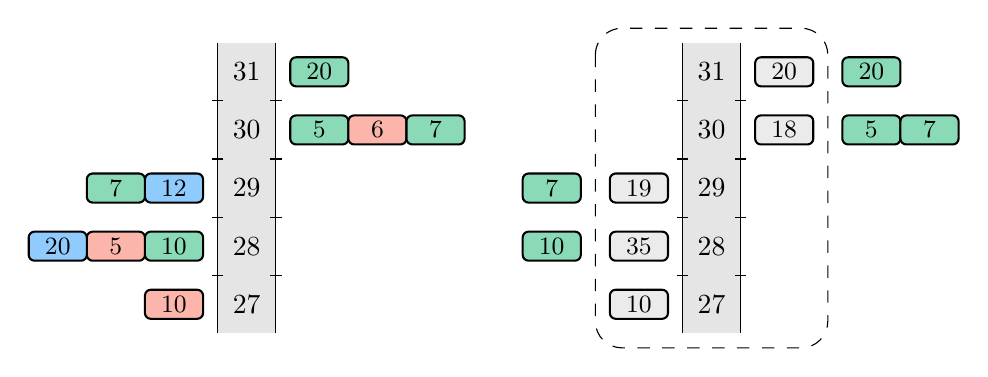
\begin{tikzpicture}[x=0.75pt,y=0.75pt,yscale=-0.7,xscale=0.7]
%uncomment if require: \path (0,300); %set diagram left start at 0, and has height of 300

%Shape: Rectangle [id:dp5489135505501248] 
\draw  [draw opacity=0][fill={rgb, 255:red, 0; green, 0; blue, 0 }  ,fill opacity=0.1 ] (140,60) -- (180,60) -- (180,260) -- (140,260) -- cycle ;
%Rounded Rect [id:dp5571720629473116] 
\draw  [fill={rgb, 255:red, 138; green, 218; blue, 184 }  ,fill opacity=1 ][line width=0.75]  (190,114) .. controls (190,111.79) and (191.79,110) .. (194,110) -- (226,110) .. controls (228.21,110) and (230,111.79) .. (230,114) -- (230,126) .. controls (230,128.21) and (228.21,130) .. (226,130) -- (194,130) .. controls (191.79,130) and (190,128.21) .. (190,126) -- cycle ;
%Straight Lines [id:da6082688802942293] 
\draw    (140,60) -- (140,260) (144,100) -- (136,100)(144,140) -- (136,140)(144,180) -- (136,180)(144,220) -- (136,220) ;
%Straight Lines [id:da9720053745263018] 
\draw    (180,60) -- (180,260) (184,100) -- (176,100)(184,140) -- (176,140)(184,180) -- (176,180)(184,220) -- (176,220) ;
%Rounded Rect [id:dp10362529279551769] 
\draw  [fill={rgb, 255:red, 251; green, 181; blue, 170 }  ,fill opacity=1 ][line width=0.75]  (230,114) .. controls (230,111.79) and (231.79,110) .. (234,110) -- (266,110) .. controls (268.21,110) and (270,111.79) .. (270,114) -- (270,126) .. controls (270,128.21) and (268.21,130) .. (266,130) -- (234,130) .. controls (231.79,130) and (230,128.21) .. (230,126) -- cycle ;
%Rounded Rect [id:dp3209795107013548] 
\draw  [fill={rgb, 255:red, 138; green, 218; blue, 184 }  ,fill opacity=1 ][line width=0.75]  (270,114) .. controls (270,111.79) and (271.79,110) .. (274,110) -- (306,110) .. controls (308.21,110) and (310,111.79) .. (310,114) -- (310,126) .. controls (310,128.21) and (308.21,130) .. (306,130) -- (274,130) .. controls (271.79,130) and (270,128.21) .. (270,126) -- cycle ;
%Rounded Rect [id:dp14006433626528436] 
\draw  [fill={rgb, 255:red, 138; green, 218; blue, 184 }  ,fill opacity=1 ][line width=0.75]  (190,74) .. controls (190,71.79) and (191.79,70) .. (194,70) -- (226,70) .. controls (228.21,70) and (230,71.79) .. (230,74) -- (230,86) .. controls (230,88.21) and (228.21,90) .. (226,90) -- (194,90) .. controls (191.79,90) and (190,88.21) .. (190,86) -- cycle ;
%Rounded Rect [id:dp23032489064391803] 
\draw  [fill={rgb, 255:red, 138; green, 218; blue, 184 }  ,fill opacity=1 ][line width=0.75]  (90,194) .. controls (90,191.79) and (91.79,190) .. (94,190) -- (126,190) .. controls (128.21,190) and (130,191.79) .. (130,194) -- (130,206) .. controls (130,208.21) and (128.21,210) .. (126,210) -- (94,210) .. controls (91.79,210) and (90,208.21) .. (90,206) -- cycle ;
%Rounded Rect [id:dp2906178876656058] 
\draw  [fill={rgb, 255:red, 143; green, 203; blue, 253 }  ,fill opacity=1 ][line width=0.75]  (90,154) .. controls (90,151.79) and (91.79,150) .. (94,150) -- (126,150) .. controls (128.21,150) and (130,151.79) .. (130,154) -- (130,166) .. controls (130,168.21) and (128.21,170) .. (126,170) -- (94,170) .. controls (91.79,170) and (90,168.21) .. (90,166) -- cycle ;
%Rounded Rect [id:dp2773205270553206] 
\draw  [fill={rgb, 255:red, 138; green, 218; blue, 184 }  ,fill opacity=1 ][line width=0.75]  (50,154) .. controls (50,151.79) and (51.79,150) .. (54,150) -- (86,150) .. controls (88.21,150) and (90,151.79) .. (90,154) -- (90,166) .. controls (90,168.21) and (88.21,170) .. (86,170) -- (54,170) .. controls (51.79,170) and (50,168.21) .. (50,166) -- cycle ;
%Rounded Rect [id:dp4559050638577514] 
\draw  [fill={rgb, 255:red, 251; green, 181; blue, 170 }  ,fill opacity=1 ][line width=0.75]  (50,194) .. controls (50,191.79) and (51.79,190) .. (54,190) -- (86,190) .. controls (88.21,190) and (90,191.79) .. (90,194) -- (90,206) .. controls (90,208.21) and (88.21,210) .. (86,210) -- (54,210) .. controls (51.79,210) and (50,208.21) .. (50,206) -- cycle ;
%Rounded Rect [id:dp12376095296435441] 
\draw  [fill={rgb, 255:red, 143; green, 203; blue, 253 }  ,fill opacity=1 ][line width=0.75]  (10,194) .. controls (10,191.79) and (11.79,190) .. (14,190) -- (46,190) .. controls (48.21,190) and (50,191.79) .. (50,194) -- (50,206) .. controls (50,208.21) and (48.21,210) .. (46,210) -- (14,210) .. controls (11.79,210) and (10,208.21) .. (10,206) -- cycle ;
%Rounded Rect [id:dp5644180007175256] 
\draw  [fill={rgb, 255:red, 251; green, 181; blue, 170 }  ,fill opacity=1 ][line width=0.75]  (90,234) .. controls (90,231.79) and (91.79,230) .. (94,230) -- (126,230) .. controls (128.21,230) and (130,231.79) .. (130,234) -- (130,246) .. controls (130,248.21) and (128.21,250) .. (126,250) -- (94,250) .. controls (91.79,250) and (90,248.21) .. (90,246) -- cycle ;
%Shape: Rectangle [id:dp5662774353889877] 
\draw  [draw opacity=0][fill={rgb, 255:red, 0; green, 0; blue, 0 }  ,fill opacity=0.1 ] (460,60) -- (500,60) -- (500,260) -- (460,260) -- cycle ;
%Rounded Rect [id:dp08118930746789832] 
\draw  [fill={rgb, 255:red, 235; green, 235; blue, 235 }  ,fill opacity=1 ][line width=0.75]  (510,114) .. controls (510,111.79) and (511.79,110) .. (514,110) -- (546,110) .. controls (548.21,110) and (550,111.79) .. (550,114) -- (550,126) .. controls (550,128.21) and (548.21,130) .. (546,130) -- (514,130) .. controls (511.79,130) and (510,128.21) .. (510,126) -- cycle ;
%Straight Lines [id:da20677085553463082] 
\draw    (460,60) -- (460,260) (464,100) -- (456,100)(464,140) -- (456,140)(464,180) -- (456,180)(464,220) -- (456,220) ;
%Straight Lines [id:da40710486463167805] 
\draw    (500,60) -- (500,260) (504,100) -- (496,100)(504,140) -- (496,140)(504,180) -- (496,180)(504,220) -- (496,220) ;
%Rounded Rect [id:dp6364145985594639] 
\draw  [fill={rgb, 255:red, 235; green, 235; blue, 235 }  ,fill opacity=1 ][line width=0.75]  (510,74) .. controls (510,71.79) and (511.79,70) .. (514,70) -- (546,70) .. controls (548.21,70) and (550,71.79) .. (550,74) -- (550,86) .. controls (550,88.21) and (548.21,90) .. (546,90) -- (514,90) .. controls (511.79,90) and (510,88.21) .. (510,86) -- cycle ;
%Rounded Rect [id:dp2804611471386602] 
\draw  [fill={rgb, 255:red, 235; green, 235; blue, 235 }  ,fill opacity=1 ][line width=0.75]  (410,194) .. controls (410,191.79) and (411.79,190) .. (414,190) -- (446,190) .. controls (448.21,190) and (450,191.79) .. (450,194) -- (450,206) .. controls (450,208.21) and (448.21,210) .. (446,210) -- (414,210) .. controls (411.79,210) and (410,208.21) .. (410,206) -- cycle ;
%Rounded Rect [id:dp24217444343409034] 
\draw  [fill={rgb, 255:red, 235; green, 235; blue, 235 }  ,fill opacity=1 ][line width=0.75]  (410,154) .. controls (410,151.79) and (411.79,150) .. (414,150) -- (446,150) .. controls (448.21,150) and (450,151.79) .. (450,154) -- (450,166) .. controls (450,168.21) and (448.21,170) .. (446,170) -- (414,170) .. controls (411.79,170) and (410,168.21) .. (410,166) -- cycle ;
%Rounded Rect [id:dp045526064729431215] 
\draw  [fill={rgb, 255:red, 235; green, 235; blue, 235 }  ,fill opacity=1 ][line width=0.75]  (410,234) .. controls (410,231.79) and (411.79,230) .. (414,230) -- (446,230) .. controls (448.21,230) and (450,231.79) .. (450,234) -- (450,246) .. controls (450,248.21) and (448.21,250) .. (446,250) -- (414,250) .. controls (411.79,250) and (410,248.21) .. (410,246) -- cycle ;
%Rounded Rect [id:dp6633295562595507] 
\draw  [fill={rgb, 255:red, 138; green, 218; blue, 184 }  ,fill opacity=1 ][line width=0.75]  (350,194) .. controls (350,191.79) and (351.79,190) .. (354,190) -- (386,190) .. controls (388.21,190) and (390,191.79) .. (390,194) -- (390,206) .. controls (390,208.21) and (388.21,210) .. (386,210) -- (354,210) .. controls (351.79,210) and (350,208.21) .. (350,206) -- cycle ;
%Rounded Rect [id:dp641336334884714] 
\draw  [fill={rgb, 255:red, 138; green, 218; blue, 184 }  ,fill opacity=1 ][line width=0.75]  (350,154) .. controls (350,151.79) and (351.79,150) .. (354,150) -- (386,150) .. controls (388.21,150) and (390,151.79) .. (390,154) -- (390,166) .. controls (390,168.21) and (388.21,170) .. (386,170) -- (354,170) .. controls (351.79,170) and (350,168.21) .. (350,166) -- cycle ;
%Rounded Rect [id:dp4238339096677155] 
\draw  [fill={rgb, 255:red, 138; green, 218; blue, 184 }  ,fill opacity=1 ][line width=0.75]  (570,114) .. controls (570,111.79) and (571.79,110) .. (574,110) -- (606,110) .. controls (608.21,110) and (610,111.79) .. (610,114) -- (610,126) .. controls (610,128.21) and (608.21,130) .. (606,130) -- (574,130) .. controls (571.79,130) and (570,128.21) .. (570,126) -- cycle ;
%Rounded Rect [id:dp3352222243665929] 
\draw  [fill={rgb, 255:red, 138; green, 218; blue, 184 }  ,fill opacity=1 ][line width=0.75]  (610,114) .. controls (610,111.79) and (611.79,110) .. (614,110) -- (646,110) .. controls (648.21,110) and (650,111.79) .. (650,114) -- (650,126) .. controls (650,128.21) and (648.21,130) .. (646,130) -- (614,130) .. controls (611.79,130) and (610,128.21) .. (610,126) -- cycle ;
%Rounded Rect [id:dp018044766031021897] 
\draw  [fill={rgb, 255:red, 138; green, 218; blue, 184 }  ,fill opacity=1 ][line width=0.75]  (570,74) .. controls (570,71.79) and (571.79,70) .. (574,70) -- (606,70) .. controls (608.21,70) and (610,71.79) .. (610,74) -- (610,86) .. controls (610,88.21) and (608.21,90) .. (606,90) -- (574,90) .. controls (571.79,90) and (570,88.21) .. (570,86) -- cycle ;
%Rounded Rect [id:dp43481833872293096] 
\draw  [dash pattern={on 4.5pt off 4.5pt}] (400,68.3) .. controls (400,58.19) and (408.19,50) .. (418.3,50) -- (541.7,50) .. controls (551.81,50) and (560,58.19) .. (560,68.3) -- (560,251.7) .. controls (560,261.81) and (551.81,270) .. (541.7,270) -- (418.3,270) .. controls (408.19,270) and (400,261.81) .. (400,251.7) -- cycle ;

% Text Node
\draw (160,80) node    {$31$};
% Text Node
\draw (160,119.5) node    {$30$};
% Text Node
\draw (210,120) node  [font=\small]  {${\textstyle 5}$};
% Text Node
\draw (160,160) node    {$29$};
% Text Node
\draw (160,200) node    {$28$};
% Text Node
\draw (160,240) node    {$27$};
% Text Node
\draw (250,120) node  [font=\small]  {$6$};
% Text Node
\draw (290,120) node  [font=\small]  {$7$};
% Text Node
\draw (210,80) node  [font=\small]  {$20$};
% Text Node
\draw (110,200) node  [font=\small]  {$10$};
% Text Node
\draw (110,160) node  [font=\small]  {$12$};
% Text Node
\draw (70,160) node  [font=\small]  {$7$};
% Text Node
\draw (70,200) node  [font=\small]  {${\textstyle 5}$};
% Text Node
\draw (30,200) node  [font=\small]  {$20$};
% Text Node
\draw (110,240) node  [font=\small]  {$10$};
% Text Node
\draw (480,80) node    {$31$};
% Text Node
\draw (480,119.5) node    {$30$};
% Text Node
\draw (530,120) node  [font=\small]  {$18$};
% Text Node
\draw (480,160) node    {$29$};
% Text Node
\draw (480,200) node    {$28$};
% Text Node
\draw (480,240) node    {$27$};
% Text Node
\draw (530,80) node  [font=\small]  {$20$};
% Text Node
\draw (430,200) node  [font=\small]  {$35$};
% Text Node
\draw (430,160) node  [font=\small]  {$19$};
% Text Node
\draw (430,240) node  [font=\small]  {$10$};
% Text Node
\draw (370,200) node  [font=\small]  {$10$};
% Text Node
\draw (370,160) node  [font=\small]  {$7$};
% Text Node
\draw (590,120) node  [font=\small]  {$5$};
% Text Node
\draw (630,120) node  [font=\small]  {$7$};
% Text Node
\draw (590,80) node  [font=\small]  {$20$};


\end{tikzpicture}

  \end{center}
\end{frame}

\begin{frame}{Limit Orderbook Examples}
  \begin{columns}[T]
    \begin{column}{0.4\textwidth}
      \begin{tabular}{|c|c|c|}
        \hline
        \textbf{Bid Qty}        & \textbf{Price}          & \textbf{Ask Qty}       \\
        \hline
        \cellcolor{gray!10}     & \cellcolor{gray!10}130  & \cellcolor{gray!10}24  \\
        \cellcolor{gray!10}     & \cellcolor{gray!10}125  & \cellcolor{gray!10}20  \\
        \cellcolor{gray!10}     & \cellcolor{gray!10}120  & \cellcolor{gray!10}10  \\
        \cellcolor{gray!10}15   & \cellcolor{gray!10}80   & \cellcolor{gray!10}    \\
        \cellcolor{gray!10}15   & \cellcolor{gray!10}75   & \cellcolor{gray!10}    \\
        \cellcolor{gray!10}30   & \cellcolor{gray!10}70   & \cellcolor{gray!10}    \\
        \hline
      \end{tabular}
    \end{column}

    \begin{column}{0.6\textwidth}
      \textbf{Discussion Questions}
      \begin{itemize}
        \item Why are all bids prices below all ask prices?
        \item Why do the quantities of quotes decrease as we approach the middle price?
        \item Would we consider this orderbook liquid?
        \item What is the market price of AMZN in this orderbook?
      \end{itemize}
    \end{column}
  \end{columns}

\end{frame}

\section{Finance Industry}

\begin{frame}{The Exchange Business Model}
  Exchanges make money by charging a fee per trade.

  This fee is usually proportional to the dollar volume of the trade.

  Exchanges benefit from high trading volume, so they have an incentive to attract participants to their platform.

  To attract customers, exchanges do the following:
  \begin{itemize}
    \item They provide a fair and transparent trading environment.
    \item Have high liquidity.
  \end{itemize}
\end{frame}

\begin{frame}{Market Markets}
  \begin{sqt:definition}
    A \textbf{market maker} is a participant in an exchange who provides liquidity by continuously quoting buy and sell prices for a security.
  \end{sqt:definition}

  Market makers must fulfill obligations to the exchange, or lose their status as a market maker.
  \begin{itemize}
    \item Quote a minimum size at all times.
    \item Quote within a certain spread.
  \end{itemize}
\end{frame}

\section{Trading \& Research}

\begin{frame}{Trading and Research Roles}
  \begin{itemize}
    \item \textbf{Trader}
    \item \textbf{Researcher}
  \end{itemize}

  \vspace{0.5cm}
  \begin{sqt:result}
    The boundaries between these two roles may across firms and teams.
  \end{sqt:result}
\end{frame}

\begin{frame}{Trader}
  TODO: get help for this slide
\end{frame}

\begin{frame}{Researcher}
  There is much more to research than just alpha and pricing theory.

  There are a wide variety of research roles, but they generally fall into the following categories:

  \begin{itemize}
    \item \textbf{Alpha}: Discovering predictive signals and trading opportunities
    \item \textbf{Pricing}: Pricing exotics (e.g. barrier options)
    \item \textbf{Risk}: Risk
    \item \textbf{Execution}: Transaction costs analysis
    \item \textbf{Portfolio Optimization}: 
  \end{itemize}

  Roles also look different depending on time-horizon.

  TODO: finish this slide later
\end{frame}

\begin{frame}{Researcher Interviews: Core Skills}
  These interviews also have probability questions.
  Also may have questions about statistics or take home projects.
\end{frame}

\section{Engineering}

\begin{frame}{Engineering Roles}

  \begin{itemize}
    \item \textbf{Software Engineer}
    \item \textbf{Quantitative Developer}
    \item \textbf{Hardware Engineer}
  \end{itemize}
\end{frame}

\begin{frame}{Software Engineering}
  In trading firms, software engineers do much of the same work as software engineers in other industries:
  \begin{itemize}
    \item \textbf{Application Development}
    \item \textbf{UI Development}
    \item \textbf{Data Engineering}
  \end{itemize}

  \begin{sqt:result}
    There isn't really a difference between the software roles.
  \end{sqt:result}
\end{frame}

\begin{frame}{Software Engineering Interviews: Core Skills}
  Fundamental competencies expected across all software roles during the interview

  \begin{itemize}
    \item \textbf{Data Structures \& Algorithms}: binary search, graphs, complexity analysis
    \item \textbf{Design Skills}: System design, API design, code design, OOP
    \item \textbf{General Knowledge}: Databases, Networks, OS, Concurrency, Compilers
    \item \textbf{Testing}: Unit tests, mock objects, designing for testability
  \end{itemize}
\end{frame}

\begin{frame}{Software Engineering Interviews: Specialized Tracks}
  Many firms separate candidates into specialized tracks early in the process.

  \vspace{0.3cm}
  \textbf{Low-Latency Track}
  \begin{itemize}
    \item C++
    \item Operating Systems
    \item Computer Architecture
  \end{itemize}

  \vspace{0.3cm}
  \textit{Example firms: Citadel Securities, QRT}
\end{frame}

\begin{frame}{Software Engineering Interviews: Specialized Tracks}
  \textbf{Python Track}
  \begin{itemize}
    \item Probability and statistics
    \item Data manipulation (NumPy, Pandas, SQL)
    \item Other stats (machine learning, data science)
  \end{itemize}

  \textit{Example firms: Citadel Securities}
\end{frame}

\begin{frame}{Quantitative Development}
  Half developer, half researcher.

  \vspace{0.3cm}
  \textbf{Math/Stats Skills}
  \begin{itemize}
    \item Undergrad math (linear algebra, probability, statistics)
    \item ML techniques (linear regression, clustering, decision trees, gradient boosting)
    \item Python for research (NumPy, Pandas, sklearn, statsmodels, plotting libraries)
  \end{itemize}

  \vspace{0.3cm}
  \textbf{Dev Skills}
  \begin{itemize}
    \item Expected to be as proficient as any other dev
  \end{itemize}

  \vspace{0.3cm}
  \textit{Example firms: Citadel Securities}
\end{frame}

\section{Resources}

\begin{frame}{Resources}
  \textbf{Trading Fundamentals Talks}
  \begin{itemize}
    \item \href{https://www.youtube.com/watch?v=hYmR5qk4z8w}{Oden Petersen \& QuantSoc - Systematic Trading Workshop}
    \item \href{https://www.youtube.com/watch?v=2YkK4DnEBRE}{George Mukun Wang \& SQT - Intro to Quant Trading}
  \end{itemize}

  \textbf{Trading Interview Prep}
  \begin{itemize}
    \item Green book
    \item Dice problems
  \end{itemize}
\end{frame}

\begin{frame}{Resources}
  \textbf{Math} (I might just be a Botev glazer)
  \begin{itemize}
    \item \textit{An Advanced Course in Probability and Stochastic Processes - Zravko Botev}
    \item \textit{Data Science and Machine Learning - Zdravko Botev}
  \end{itemize}
\end{frame}

\begin{frame}{Resources}
  \textbf{Software Engineering Classics}
  \begin{itemize}
    \item \textit{Designing Data-Intensive Applications} (DDIA)
    \item \textit{Operating Systems: Three Easy Pieces} (OSTEP)
  \end{itemize}

  \textbf{C++ Classics}
  \begin{itemize}
    \item \textit{Exceptional C++} by Herb Sutter
    \item \textit{Effective Modern C++} by Scott Meyers
  \end{itemize}

  \textbf{Blogs, Websites, Videos}
  \begin{itemize}
    \item \href{https://agner.org}{Agner Fog Website}
  \end{itemize}
\end{frame}

\end{document}